
 
\chapter{Heaps}
\section{Introduction}
A heap is a special kind of complete binary tree.  The key property of a heap is that  the target element (the minimum or the maximum) is always stored at the root of the heap.   This is done by reordering the nodes to ensure that the property is true.   A heap can be one of two types, a max heap where the parent node is greater than its children, or a min heap where the parent node is smaller than its children.

To be a valid heap, every element has to follow the heap rule. For max heaps the rule is: \begin{equation}value(parent) \geq value(child)\end{equation}   and for a min heap the rule is: \begin{equation}value(parent) \leq value(child)\end{equation}

A heap is considered to be a partially ordered data structure because the elements within any given level have no defined ordering.  Heaps are commonly used as the implementation for a priority queue.

\begin{figure}[H]
\centering
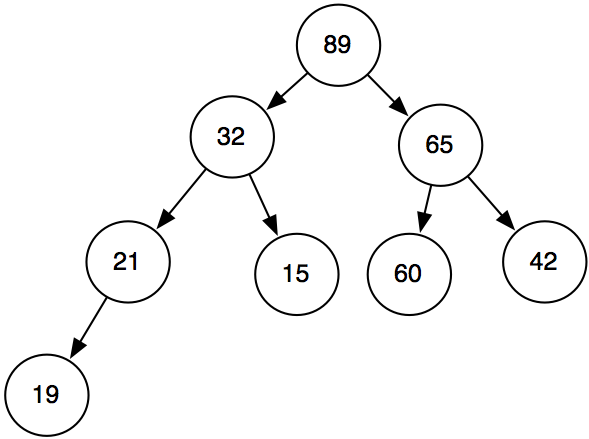
\includegraphics{pictures/maxheap.png}
\label{fig:maxheap}
\caption{A max heap.  Notice that the sibling nodes have no ordering within the level}
\end{figure}


\section{Operations}
A heap should provide the functionality to insert, delete, and retrieve the min/max value.    Additionally the heap must provide the standard data structure operations of create, destroy and isEmpty.   A robust heap library should allow the library user to choose between min or max heap capabilities when the heap is created.  The minimum set of operations is shown below.  

\begin{itemize}
\item insert
\item delete
\item findMinorMax
\item isEmpty
\item create
\item destroy
\end{itemize}

The Heap ADT requires the same abstraction with void * pointers,   operations to create nodes,  and function pointers to compare, delete and print data as the previous ADTs we have studied.     The create, destroy, and isEmpty functions are very similar to the same functions for other ADTs and are not explained in detail here.

The insert and delete functions for a heap are the most complicated operations.   

\subsection{Heap Insert}

A heap is a specialized version of a complete tree.  This means that all insertions must occur at the left-most side of the bottom level of the tree in order to maintain the property of completeness.   The algorithm for adding an element to a heap follows:
\begin{lstlisting}
insert(Heap * heap, void * data)
{
    create a node from the data
    locate the next position in the heap (the left most position with no node)
    add the new node to the located position
    reheapify the heap to maintain the heap property
}
\end{lstlisting}

The process of reheapification consists of swapping elements until the heap property is satisfied or until the root of the heap is reached.  The pseudocode for reheapification is shown below.

\begin{lstlisting}
reheapify(Heap * heap, Node * newNode)
{
     parentNode = get parent node of newNode
     while(newNode->data is greater than parentNode->data  //or less than for a min heap
     {
     	swap positions of newNode and Parent Node
     	parentNode = get parent node of newNode (has changed because of the swap)
     }
}
 \end{lstlisting}
 
\subsection{Heap Delete}
 
 The most common way to delete elements from a heap is to remove the value at the root node as part of the the findMinorMax operation.
 To remove the root node,  you find the left-most leaf of the heap,  replace the root node with that node, and then reheapify downwards until the heap property is satisfied.
 
 \begin{lstlisting}
 void * findAndDeleteRoot(Heap * heap)
 {
 	tempNode = heap->rootNode
 	heap->rootNode = the node in the "last" position in the tree //the leftmost, bottom node
 	outOfPlacePtr = heap->rootNode  // keep track of the node that you're moving into place
 	remove the node in the last position //after copying it into the root
 	while ( outOfPlacePtr->data is less than either left or right child)  //or greater than for a min heap
 	{
 		swap outOfPlacePtr and child with greatest value
 	}
 	return tempNode->data
 }
 \end{lstlisting}
 
 The delete process for the root node can be used to delete any node in the heap.   The node to be deleted is the root node of a subtree,  and the delete algorithm can be applied to the subtree instead of the entire heap.
 
\section{Array Implementation of a Heap}

Heaps can be implemented using a Binary Tree ADT.  However,  the property that a heap is a complete binary tree allows a heap to be implemented using an array.  The array implementation removes the need for pointers as the positions of the child nodes can be easily calculated.   The first empty position in the array is the next position to be filled.

\begin{figure}[H]
\centering
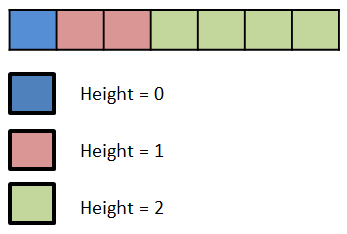
\includegraphics{pictures/heap0.png}
\label{fig:heap0}
\end{figure}

The array is organized so index 0 is height 0, height 1 is indexes 1-2, height 2 is indexes 2-5 and so on.   The swaps necessary for inserting or deleting elements can be accomplished simply by calculating the appropriate array index.

\subsection{Adding Elements}

Adding an element to a heap has a worst case complexity of O(height) or O(log(N)), since there is a maximum of 1 swap per level of the heap.
The algorithm for inserting elements does not change when an array is used for implementation.  Only the implementation details change.   Consider the following example where 10, 23, 3, 32, 17 and 5 are added to a max heap.

We begin by adding 10 to an empty heap.

\begin{figure}[H]
\centering
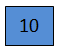
\includegraphics{pictures/heap1.png}
\label{fig:heap1}
\end{figure}

\begin{figure}[H]
\centering
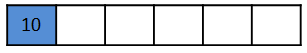
\includegraphics{pictures/heap1a.png}
\label{fig:heap1a}
\end{figure}

10 is added as the root of the heap at position 0 in the array.   It is the first level of the binary tree.  
We then add 23 to the heap.

\begin{figure}[H]
\centering
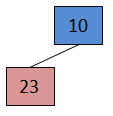
\includegraphics{pictures/heap2.png}
\label{fig:heap2}
\end{figure}

\begin{figure}[H]
\centering
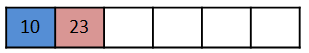
\includegraphics{pictures/heap2a.png}
\label{fig:heap2a}
\end{figure}

First, 23 is added as 10's child.  It is placed in the first empty left-most position in the tree, which is also the first empty position in the array.
Because 23 is greater than 10,  the heap must be reheapified.  

\begin{figure}[H]
\centering
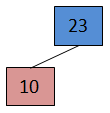
\includegraphics{pictures/heap3.png}
\label{fig:heap3}
\end{figure}

\begin{figure}[H]
\centering
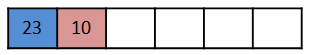
\includegraphics{pictures/heap3a.png}
\label{fig:heap3a}
\end{figure}

23 is compared to its parent value (10).  23 is larger so the two values are swapped and 23 is the new root of the heap.  10 is the child of 23.   We then add 3 to the heap.   

\begin{figure}[H]
\centering
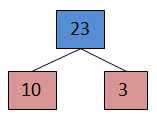
\includegraphics{pictures/heap4.png}
\label{fig:heap4}
\end{figure}

\begin{figure}[H]
\centering
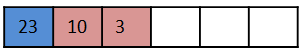
\includegraphics{pictures/heap4a.png}
\label{fig:heap4a}
\end{figure}

3 is added as the second child of 23.   It is added in position 2 of the array.   3 is compared to the value of its parent (23).  3 is smaller than its parent value so no swap is needed.   We then add 32 to the heap.

\begin{figure}[H]
\centering
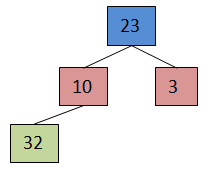
\includegraphics{pictures/heap5.png}
\label{fig:heap5}
\end{figure}

\begin{figure}[H]
\centering
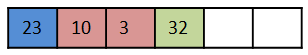
\includegraphics{pictures/heap5a.png}
\label{fig:heap5a}
\end{figure}

32 is added at the next, left-most position in the heap (the first empty position in the array).  32 is compared with its parent value (10).  32 is larger than 10 so the two values must be swapped.

\begin{figure}[H]
\centering
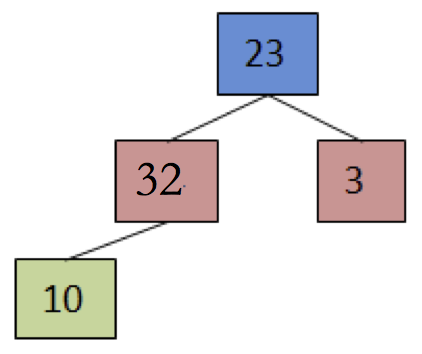
\includegraphics{pictures/heap6.png}
\label{fig:heap6}
\end{figure}

\begin{figure}[H]
\centering
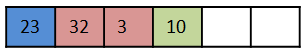
\includegraphics{pictures/heap6a.png}
\label{fig:heap6a}
\end{figure}

32 iis not the root of the heap, so we again compare 32  with its parent value (23).   32 is larger than 23, so a swap must be made.

\begin{figure}[H]
\centering
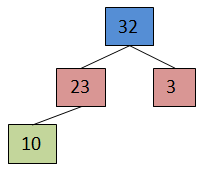
\includegraphics{pictures/heap7.png}
\label{fig:heap7}
\end{figure}

\begin{figure}[H]
\centering
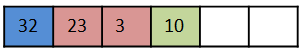
\includegraphics{pictures/heap7a.png}
\label{fig:heap7a}
\end{figure}

32 is the new root of the heap so no further comparisons are necessary.   We then add 17 to the heap.

\begin{figure}[H]
\centering
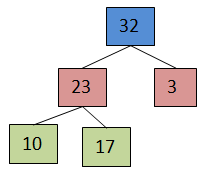
\includegraphics{pictures/heap8.png}
\label{fig:heap8}
\end{figure}

\begin{figure}[H]
\centering
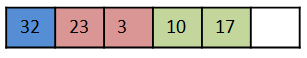
\includegraphics{pictures/heap8a.png}
\label{fig:heap8a}
\end{figure}

17 is added as a child of 23 to the first, left-most empty position in the tree.  17 is compared to the value of its parent(23).  17 is smaller than its parent value so no swap is required.   We then add 5 to the heap.

\begin{figure}[H]
\centering
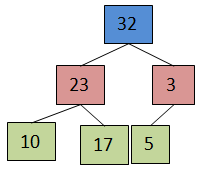
\includegraphics{pictures/heap9.png}
\label{fig:heap9}
\end{figure}

\begin{figure}[H]
\centering
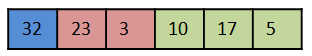
\includegraphics{pictures/heap9a.png}
\label{fig:heap9a}
\end{figure}

5 is added to the next position in the heap, as the first child of 3.    5 is compared to its parent value (3).  5 is larger than three so the two values must be swapped.

\begin{figure}[H]
\centering
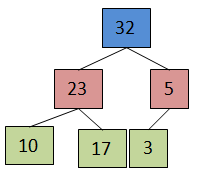
\includegraphics{pictures/heap10.png}
\label{fig:heap10}
\end{figure}

\begin{figure}[H]
\centering
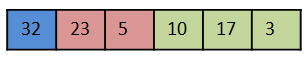
\includegraphics{pictures/heap10a.png}
\label{fig:heap10a}
\end{figure}

Finally 5 is compared to its new parent (32).  5 is smaller than 32 so no swap is necessary.

It can be seen that the final array representation is not fully sorted, and not fully segregated by value ranges (5 has a height of 1, higher than 10 and 17).   Nonetheless the heap rule holds and the partial ordering of the heap can easily be maintained by swaps.



\subsection{Removing Elements}

Elements of a heap are generally removed from the root, or the largest/smallest element in the structure. The root is then filled with the most recent added element , and the heap is resorted by swapping with the larger child until it satisfies the heap property.   If it is necessary to remove an interior item from a heap,  the subtree rooted in the item to be removed is handled in the same fashion as the entire heap.


Removing an element will always result in a complete tree because only leaf nodes are actually removed after the value is swapped in to a new spot.

The complexity of a deletion is O(height) or O(log(N)) since there is a maximum of 1 swap necessary per height.

\begin{figure}[H]
\centering
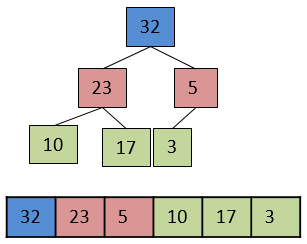
\includegraphics{pictures/heap11.png}
\label{fig:heap11}
\caption{The Starting Heap}
\end{figure}

\begin{figure}[H]
\centering
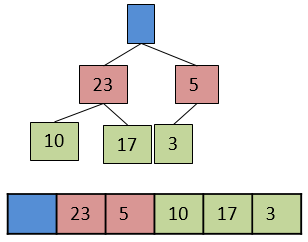
\includegraphics{pictures/heap12.png}
\label{fig:heap12}
\end{figure}

The root is removed, leaving an empty spot in the heap.

\begin{figure}[H]
\centering
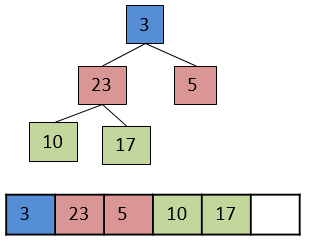
\includegraphics{pictures/heap13.png}
\label{fig:heap13}
\end{figure}

The most recently added element is copied to the root position.   The most recently added node is deleted.  The new root node(3) is compared to both of its child nodes (23, and 5).   3 is less than at least one of its children so it must be swapped.   
The heap does not follow the heap rule, a sort must be done.

\begin{figure}[H]
\centering
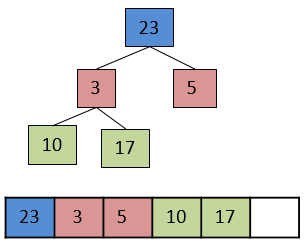
\includegraphics{pictures/heap14.png}
\label{fig:heap14}
\end{figure}

3 is swapped with the larger child, 23.  3 is now compared with its new children (10 and 17).    3 is smaller than at least one child, therefor the heap still does not satisfy the heap property.  Another swap must be performed.

\begin{figure}[H]
\centering
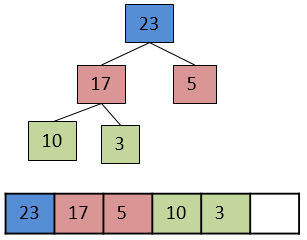
\includegraphics{pictures/heap15.png}
\label{fig:heap15}
\end{figure}

3 is swapped with the larger child, 17. The heap property is now satisfied.


\section{Extending Activities}

\begin{itemize}
\item Develop a formula to calculate the position of a parent node in an array-implementation of a heap.  The only input information to the formula is the position of the current node.
\item Create the C struct for a binary-tree based heap.  Your struct should have members for the heap,  the last added element, the next position, and function pointers to manipulate void* data.
\item Heaps do not have to be binary trees.   Many variations of heaps are possible.   Use internet resources to learn about one of the following different types of heaps:  skew heaps, binomial heap, or leftist heap.   Write the pseudocode for insert and delete operations for the type of heap you chose.
\item The complexity of insert and delete for a binary heap is O(log(N)).   Why is that?  Create a written explanation, chart, or diagram that explains why log(N) is the complexity for those operations.

\end{itemize}